\chapter{ПРОЕКТИРОВАНИЕ И ПРОГРАММНАЯ РЕАЛИЗАЦИЯ СИСТЕМЫ}
\label{ch:проектирование_и_программная_реализация_системы}

\section{Архитектура клиентского приложения}
\label{sec:архитектура_клиентского_приложения}

Проектирование системы осуществлялось в соответствии с парадигмой \textit{Edge AI}, предполагающей перенос вычислительной нагрузки непосредственно на устройство конечного пользователя~\cite{xu2024ondevice}. Весь цикл вывода модели --- от токенизации до формирования вероятностного прогноза --- протекает внутри изолированного контура браузера без обращения к какому-либо внешнему серверу~\cite{ruan2024webllm}. Архитектурная схема строится на строгом разграничении ответственности между тремя логическими уровнями: уровнем представления (\textit{Presentation Layer}), реализующим управление состоянием средствами \textit{React}; уровнем оркестрации (\textit{Orchestration Layer}), организующим конвейер обработки через \textit{Transformers.js}; и вычислительным ядром (\textit{Computation Layer}), где тензорные операции транслируются в машинный код посредством \textit{ONNX Runtime Web}~\cite{wang2024anatomizing}. Подобная декомпозиция обеспечивает независимую эволюцию каждого слоя и создаёт предпосылки для воспроизводимого экспериментального тестирования.

Приложение организовано как одностраничное \textit{SPA} с двумя функционально обособленными представлениями, переключаемыми посредством типа \texttt{AppTab~=~"playground"~|~"benchmark"} в компоненте \textit{Header}. Первое --- \textit{Playground} (\texttt{PlaygroundView}) --- предназначено для интерактивной классификации произвольного текста: результат отображается в виде карточки с предсказанной меткой тональности, показателем уверенности (\textit{confidence score}), задержкой вывода модели и объёмом потреблённой памяти. Второе --- \textit{Benchmark Lab} (\texttt{BenchmarkView}) --- трансформирует приложение в лабораторный стенд: пользователь загружает стандартизированный \textit{JSON}-датасет, запускает серию классификаций и наблюдает агрегированные результаты непосредственно в интерфейсе; экспорт в \textit{CSV} доступен как опциональный шаг~\cite{wang2024anatomizing}. На рисунке~\ref{fig:интерфейс-режима-классификации} представлен интерфейс режима \textit{Playground} после классификации арабскоязычного текста моделью \textit{DistilBERT Fine-tuned}: предсказанная метка \textit{Positive} зафиксирована с уверенностью 95\% при задержке вывода 98~мс.

\begin{figure}[htbp]
    \centering
    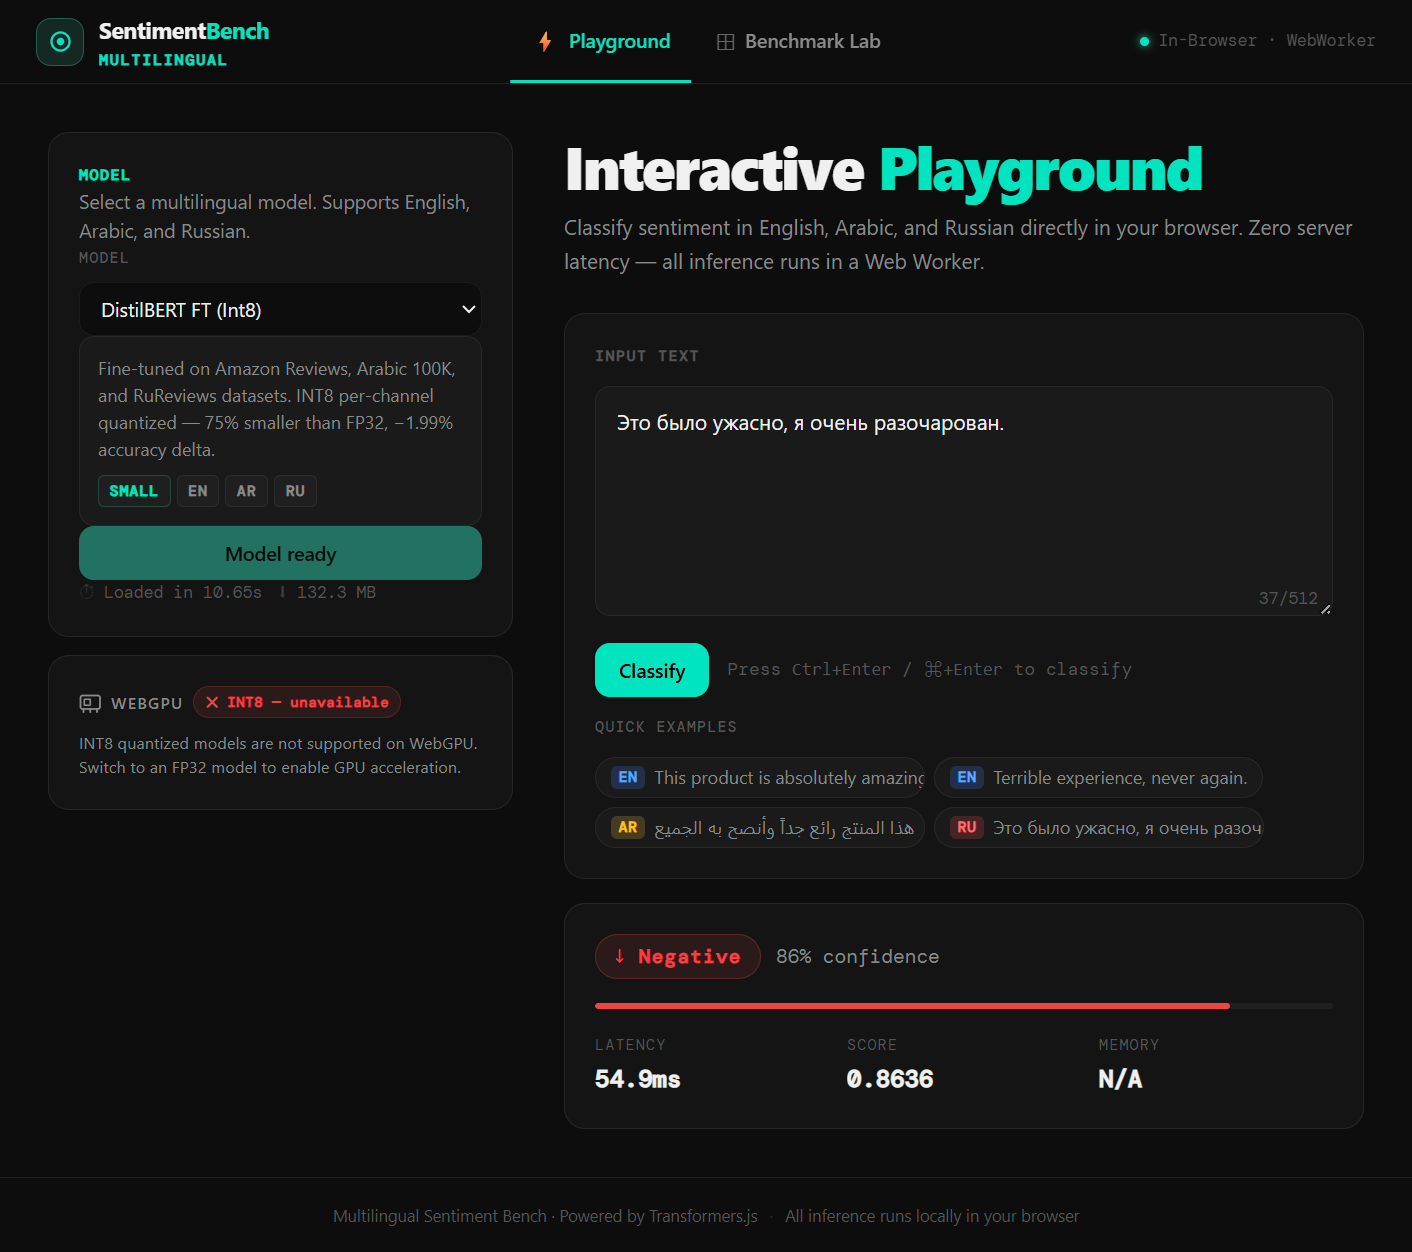
\includegraphics[width=0.95\textwidth]{images/интерфейс-режима-классификации.png}
    \caption{Интерфейс режима \textit{Playground} с результатом классификации}
    \label{fig:интерфейс-режима-классификации}
\end{figure}

Оба представления монтируются в корневой компонент \textit{App}, обёрнутый в \textit{ClassifierProvider} --- провайдер глобального контекста, экспортирующий состояние модели и методы взаимодействия с вычислительным ядром. Интерфейс контекста \texttt{ClassifierContextValue} декларирует строго типизированный контракт: поле \texttt{loadState} типа \texttt{ModelLoadState} описывает жизненный цикл модели через четыре поля --- \texttt{status}~типа~\texttt{ModelLoadStatus} (\texttt{idle~|~loading~|~ready~|~error}), числовой прогресс загрузки \texttt{progress}, строку \texttt{statusText} для отображения в \texttt{ProgressBar}, а также опциональное поле \texttt{error}. Поля \texttt{modelLoadTimeMs} и \texttt{modelSizeMb} фиксируют телеметрию «холодного старта», получаемую из сообщения \texttt{MODEL\_READY}. Помимо этого, контекст предоставляет поля управления состоянием \textit{WebGPU}: \texttt{webGpu~:~WebGpuState}, \texttt{setWebGpuEnabled} и флаг \texttt{webGpuBlockedByDtype}, блокирующий аппаратное ускорение при несовместимом типе квантования выбранной модели~\cite{wang2024anatomizing}. Методы \texttt{loadModel} и \texttt{classify} выступают единственными точками входа для взаимодействия компонентов с фоновым потоком, полностью скрывая детали асинхронного протокола \textit{Web Worker} от уровня представления.

Вычислительное ядро сосредоточено в модуле \texttt{classifier.worker.ts}: функция \texttt{getPipelineInstance} реализует паттерн «Одиночка» (\textit{Singleton}), удерживая единственный активный экземпляр \textit{TextClassificationPipeline} в замыкании модуля и переиспользуя его на протяжении всего сеанса, --- что исключает повторную компиляцию вычислительного графа при последовательных запросах~\cite{wang2024anatomizing}. Функция принимает три аргумента: идентификатор модели \texttt{modelId}, булев флаг \texttt{useWebGpu} и колбэк для трансляции прогресса. Флаг \texttt{useWebGpu} определяет, какой из двух доступных бэкендов будет инициализирован: при значении \texttt{true} конвейер запускается на \textit{WebGPU}-бэкенде, при \texttt{false} --- на \textit{WASM}-бэкенде~\cite{ruan2024webllm}. Выбор бэкенда при инициализации отображён в диаграмме последовательности (шаги 14--17, ветка \texttt{useWebGpu = true / false}).

Перед монтированием интерфейса \textit{ClassifierContext} выполняет зондирование \texttt{navigator.gpu} посредством асинхронной функции \texttt{detectWebGpu()}, возвращающей значение типа \texttt{WebGpuStatus~=~"checking"~|~"supported"~|~"unsupported"}. Результат зондирования отражается в интерфейсном компоненте \texttt{WebGpuPanel}, предоставляющем пользователю переключатель активации \textit{WebGPU}; при недоступности \textit{WebGPU} переключатель блокируется. Компонент \texttt{WebGpuPanel} монтируется как в \texttt{PlaygroundView}, так и в \texttt{BenchmarkView}, обеспечивая единое управление бэкендом в обоих режимах работы~\cite{jia2024empowering}.

Архитектурная изоляция памяти фонового потока от \textit{DOM}-дерева обусловливает необходимость строго формализованного протокола обмена данными, описанного посредством дискриминированных объединений типов (\textit{discriminated unions}) в модуле \texttt{src/types/index.ts}. Тип \texttt{WorkerInbound} объединяет две команды: \texttt{LOAD\_MODEL} и \texttt{CLASSIFY}. Команда \texttt{LOAD\_MODEL} несёт два поля --- \texttt{modelId} и \texttt{useWebGpu:~boolean}, передавая воркеру не только идентификатор модели, но и выбранный пользователем режим аппаратного ускорения. Команда \texttt{CLASSIFY} несёт уникальный идентификатор запроса \texttt{id} для сопоставления ответа с ожидающим \textit{Promise}. Тип \texttt{WorkerOutbound} включает четыре сообщения: \texttt{MODEL\_READY}, \texttt{PROGRESS}, \texttt{CLASSIFICATION\_RESULT} и \texttt{ERROR}~\cite{ruan2024webllm}. Телеметрия латентности формируется исключительно внутри фонового потока: таймер \texttt{performance.now()} запускается перед прогоном тензоров через вычислительный граф и останавливается после получения логитов, до применения функции \textit{Softmax}, --- что исключает из измерения накладные расходы на сериализацию сообщений и реактивный рендеринг \textit{React}~\cite{wang2024anatomizing}. Снимок потребления памяти кучи \textit{JavaScript} (\texttt{usedJSHeapSize}) фиксируется функцией \texttt{getMemoryMB()} через \texttt{performance.memory} сразу после завершения вывода модели; возвращаемый тип \texttt{number~|~null} допускает отсутствие данного \textit{API} на отдельных платформах.

\begin{figure}[htbp]
    \centering
    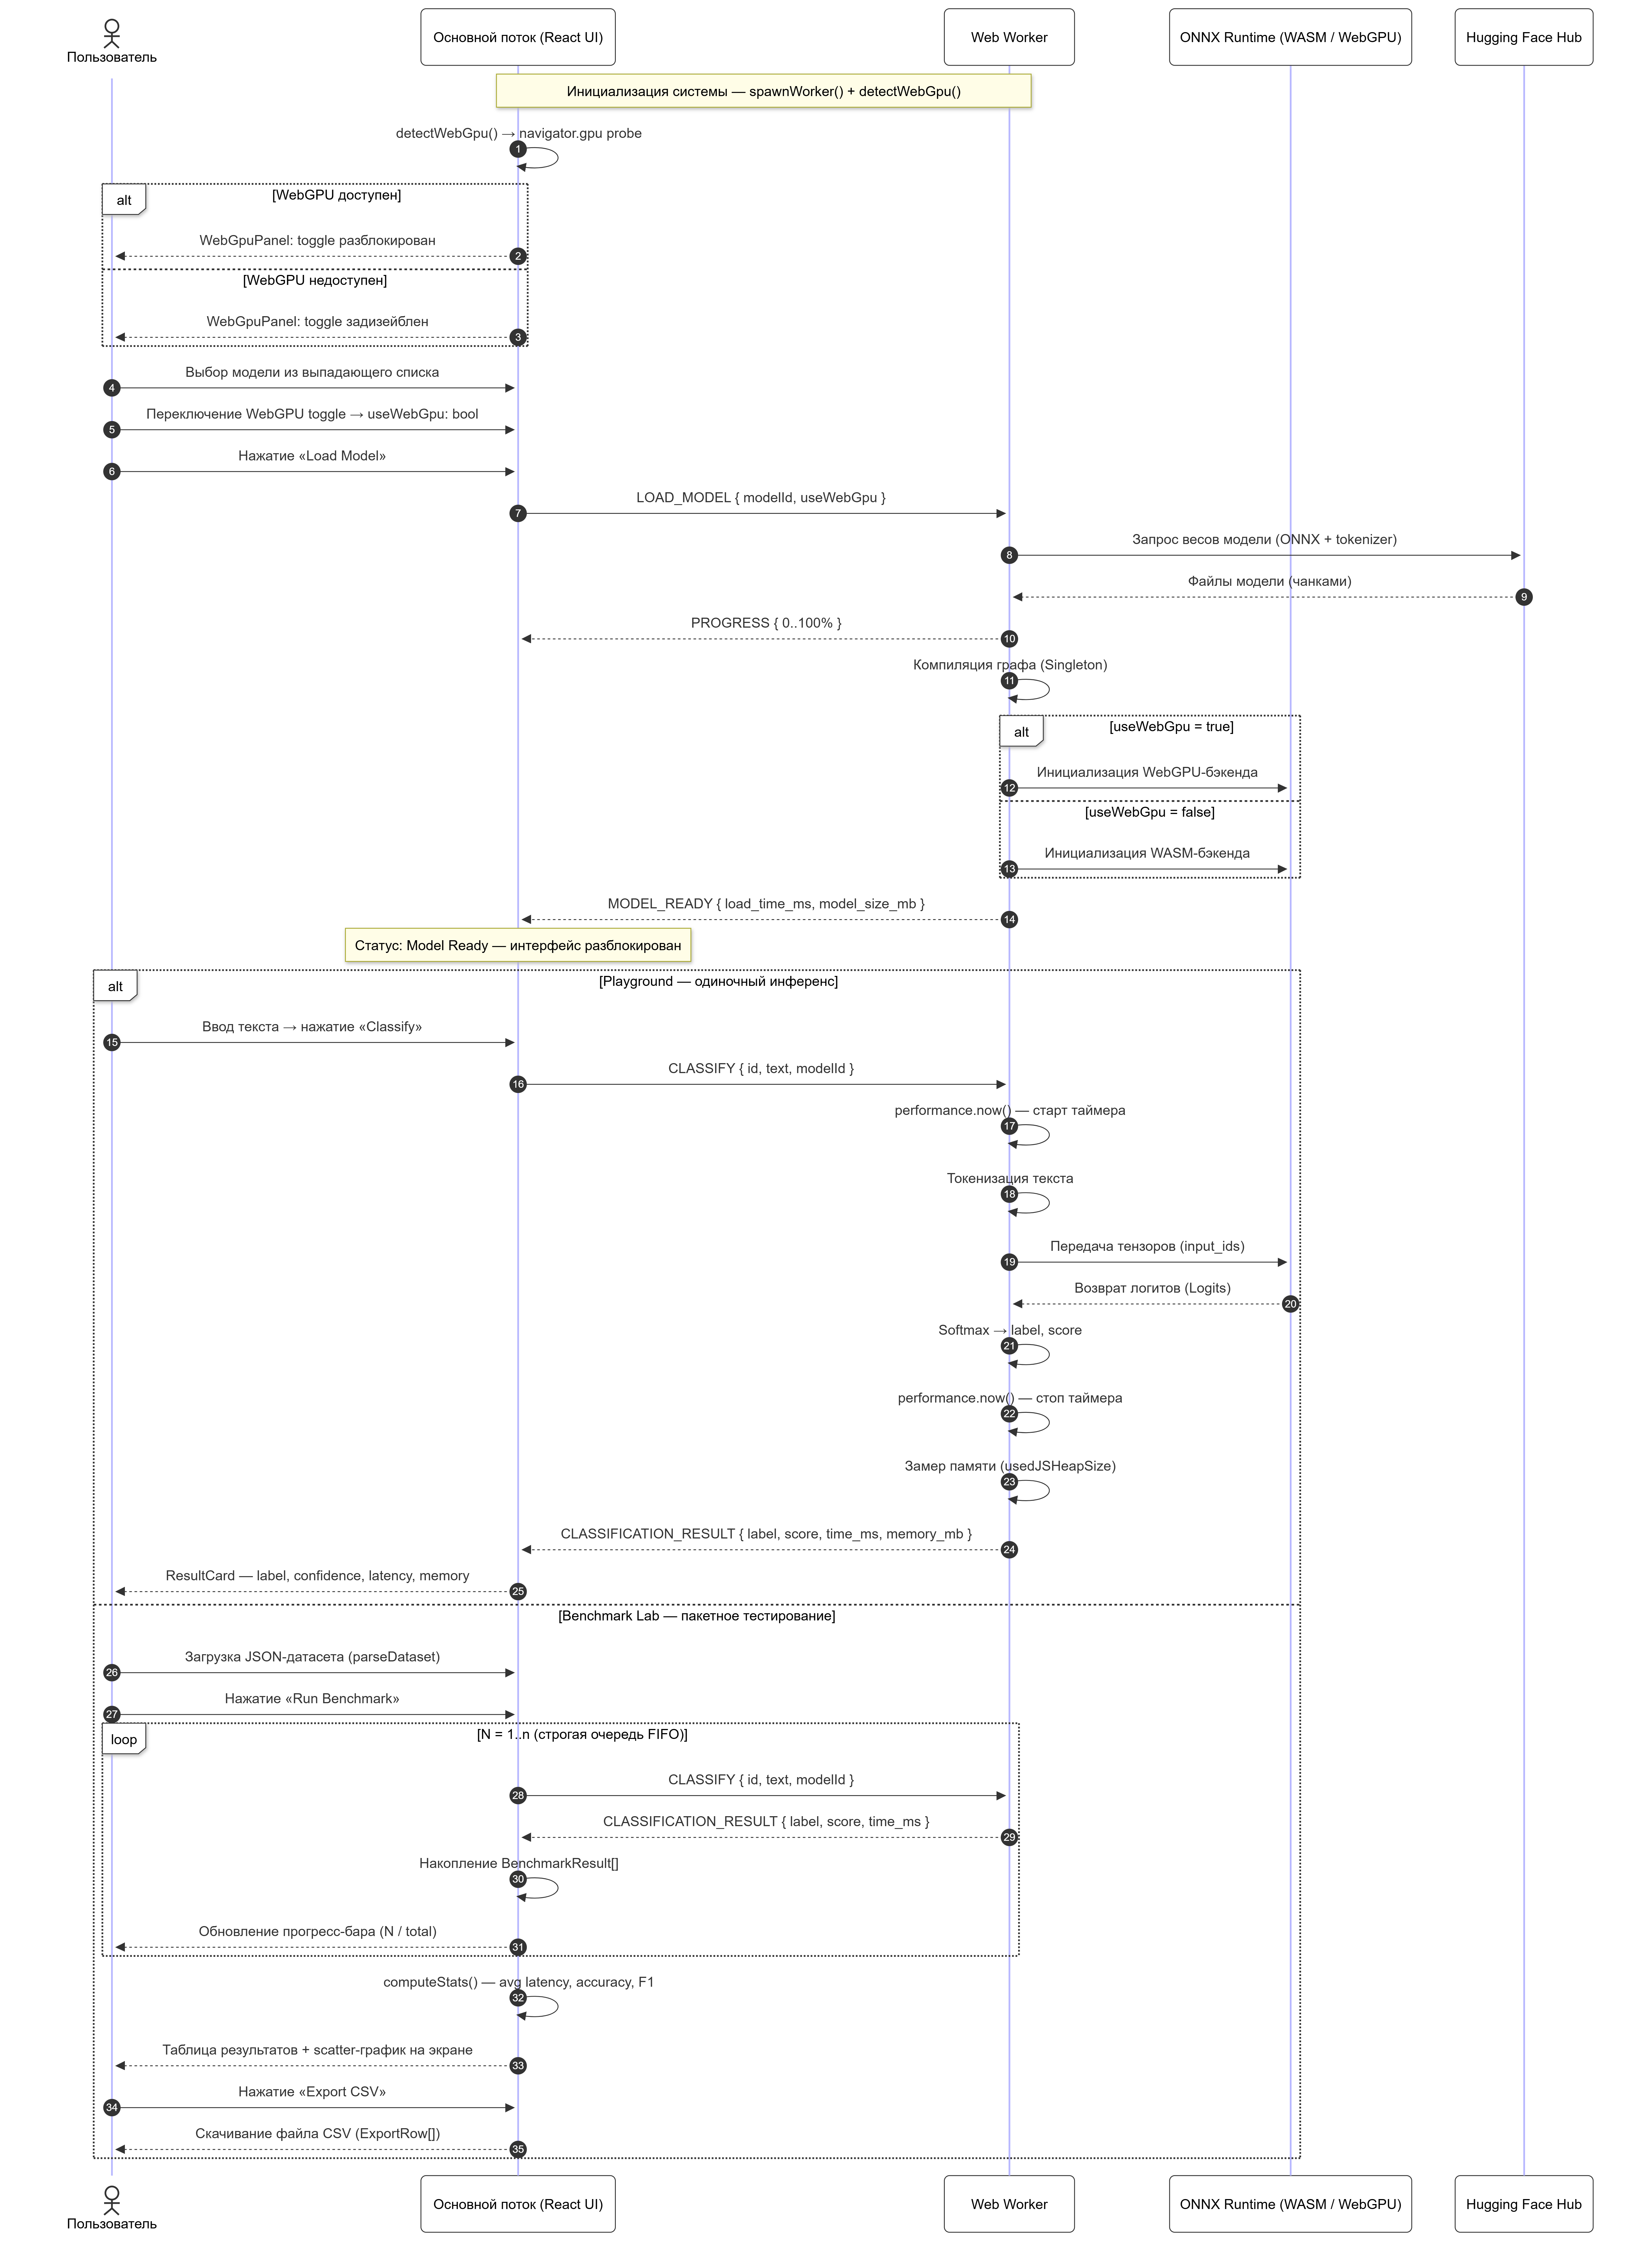
\includegraphics[width=0.95\textwidth]{images/диаграмма-последовательности-клиентского-инференса-в-браузерной-среде.png}
    \caption{Диаграмма последовательности клиентского инференса в браузерной среде}
    \label{fig:диаграмма-последовательности-клиентского-инференса-в-браузерной-среде}
\end{figure}

Полный цикл взаимодействия компонентов отображён на рисунке~\ref{fig:диаграмма-последовательности-клиентского-инференса-в-браузерной-среде}. При инициализации системы выполняются две параллельные операции: зондирование \textit{WebGPU} (\texttt{detectWebGpu}) и запуск воркера (\texttt{spawnWorker}). По команде \texttt{LOAD\_MODEL} воркер загружает веса с \textit{Hugging Face Hub} чанками, транслируя сообщения \texttt{PROGRESS}, компилирует граф и удерживает единственный экземпляр конвейера посредством \textit{Singleton}; в зависимости от флага \texttt{useWebGpu} инициализируется либо \textit{WebGPU}-бэкенд, либо \textit{WASM}-бэкенд. В режиме \textit{Playground} воркер выполняет токенизацию, прогон тензоров через граф \textit{ONNX Runtime} и постобработку логитов; в режиме \textit{Benchmark Lab} алгоритм строгой сериализации \textit{FIFO} гарантирует, что вывод модели для образца $N+1$ инициируется исключительно после полной фиксации метрик образца $N$~\cite{jia2024empowering}.

Реестр поддерживаемых моделей централизован в модуле \texttt{src/lib/models.ts}. Каждая запись описывается интерфейсом \texttt{ModelConfig}, декларирующим идентификатор репозитория на \textit{Hugging Face Hub}, наименование, перечень поддерживаемых языков, весовую категорию (\texttt{ModelSize~=~"small"~|~"medium"~|~"large"}), тип задачи (\texttt{ModelTask}), а также опциональные поля \texttt{onnxFile} и \texttt{dtype} для явного указания конкретного артефакта и типа квантования. Тип квантования объявлен как \texttt{ModelDtype~=~"fp32"~|~"q8"} и закреплён за каждой конфигурацией модели статически в реестре; воркер разрешает параметры загрузки посредством функции \texttt{getModelById(modelId)}, не получая \texttt{dtype} через интерфейс сообщений. Подобная схема позволяет подключать произвольные модели без изменения вычислительного ядра~\cite{husom2025sustainable}. На рисунке~\ref{fig:реестр-нейросетевых-моделей} отображён выпадающий список выбора модели, формируемый на основе централизованного реестра.

\begin{figure}[htbp]
    \centering
    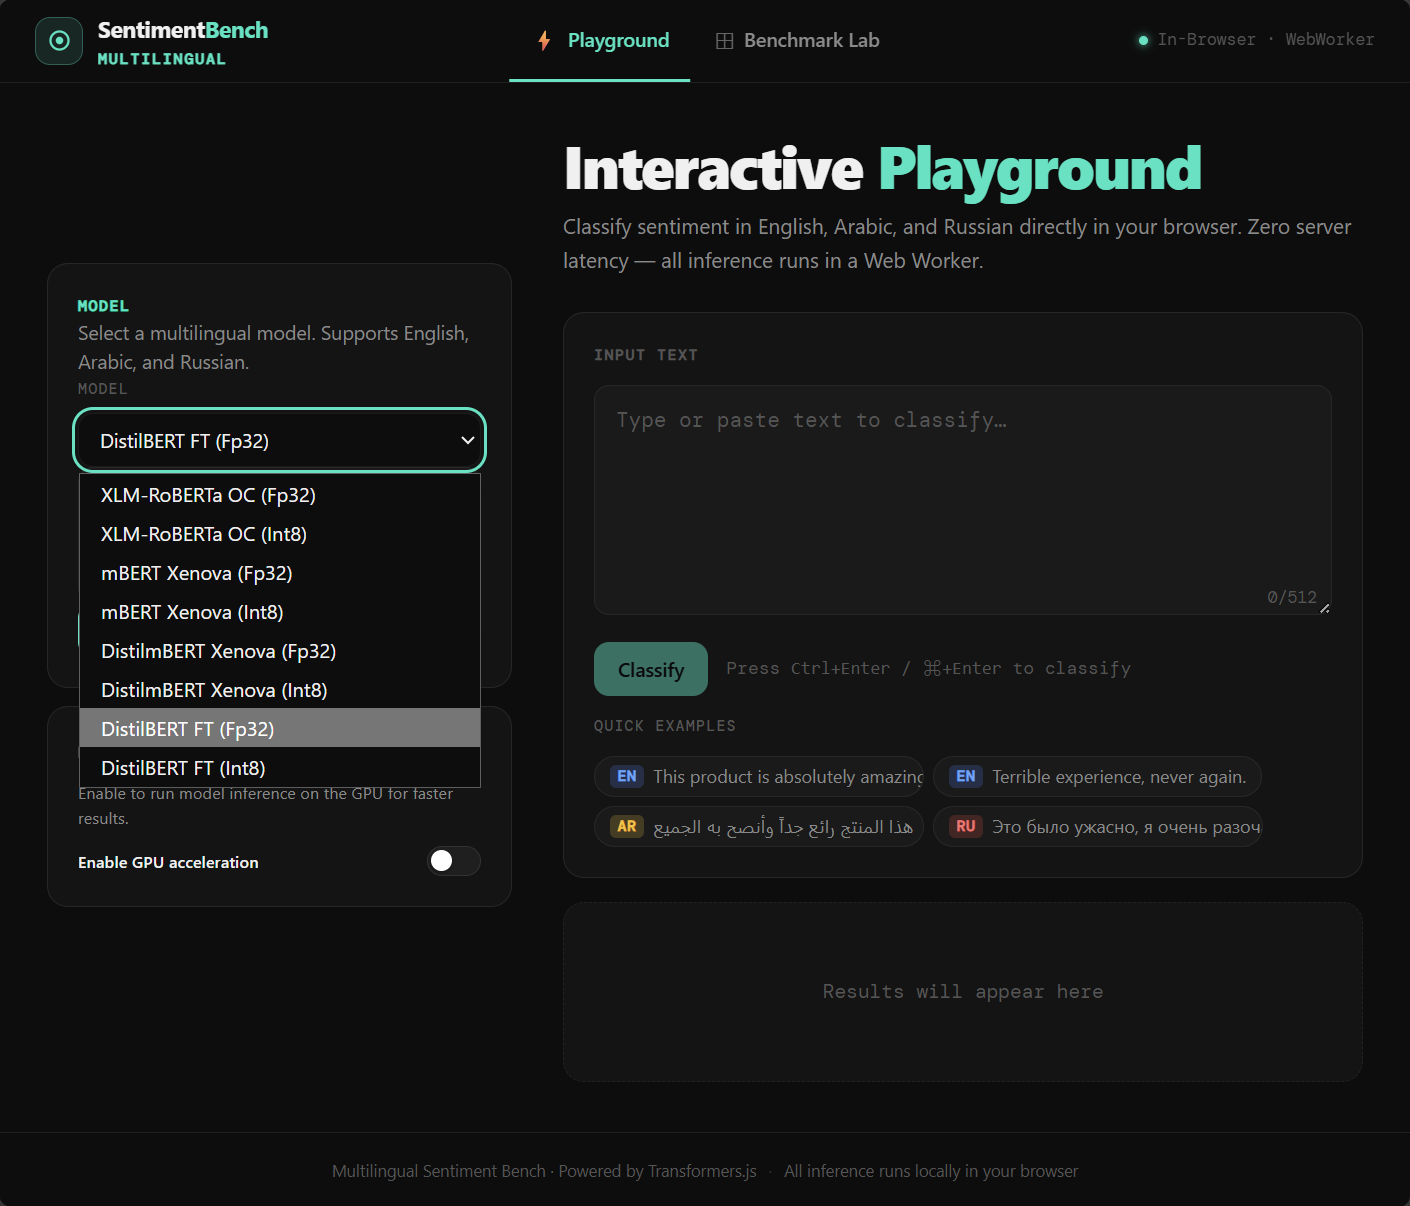
\includegraphics[width=0.95\textwidth]{images/реестр-нейросетевых-моделей.png}
    \caption{Реестр нейросетевых моделей в интерфейсе выбора конфигурации}
    \label{fig:реестр-нейросетевых-моделей}
\end{figure}

В экспериментальной части задействованы три архитектуры: \textit{Xenova/bert-base-multilingual-uncased-sentiment} в режиме \texttt{fp32} в качестве опорной конфигурации; \textit{Xenova/distilbert-base-multilingual-cased-sentiments-student} с квантованием \texttt{q8} как основной объект клиентской валидации; \textit{cardiffnlp/twitter-xlm-roberta-base-sentiment} для оценки архитектуры \textit{XLM-RoBERTa}. Дообученный вариант \textit{ayayousef/distilbert-multilingual-sentiment-finetuned} регистрируется в том же реестре и подключается к стенду идентично предобученным аналогам~\cite{sanh2019distilbert}. Функция \texttt{normalizeLabel}, импортируемая в \texttt{classifier.worker.ts} из \texttt{src/lib/models.ts}, транслирует разнородные метки различных моделей в единое перечисление \texttt{SentimentLabel~=~"POSITIVE"~|~"NEGATIVE"~|~"NEUTRAL"}, устраняя семантическую неоднородность вывода при кросс-модельном сравнении.


\section{Подготовка и конвертация нейросетевых моделей для веб-среды}
\label{sec:подготовка_и_конвертация_нейросетевых_моделей_для_веб_среды}

Перенос трансформерных архитектур в браузерную среду диктует многоступенчатый конвейер подготовки: дообучение на целевых языковых корпусах, конвертацию в формат \textit{ONNX}, квантование параметров и публикацию артефактов в реестре \textit{Hugging Face Hub} для потоковой загрузки непосредственно в браузере~\cite{xu2024ondevice, ruan2024webllm}.

Для эмпирической оценки отобраны три конфигурации, представляющие разные точки компромисса между выразительной способностью и вычислительной стоимостью. \textit{Xenova/bert-base-multilingual-uncased-sentiment} --- архитектура \textit{BERT-Base Multilingual} с~${\sim}110$~млн параметров и охватом 104~языков --- задаёт верхнюю границу предиктивного качества при максимальных ресурсных требованиях~\cite{krasitskii2025sentiment, hasan2024ensemble}. \textit{Xenova/distilbert-base-multilingual-cased-sentiments-student}, полученный посредством дистилляции знаний (\textit{knowledge distillation})~\cite{sanh2019distilbert, xu2024distillation}, декларирует сокращение параметрной ёмкости на~40\% и ускорение до~60\% при сохранении свыше~95\% качества --- данная конфигурация выступает основным объектом клиентской валидации. \textit{Cardiffnlp/twitter-xlm-roberta-base-sentiment}, дообученная на мультиязычных данных микроблогов, обеспечивает устойчивость к коллоквиальной лексике~\cite{li2024multilingual}. Совокупность трёх архитектур позволяет верифицировать гипотезу о достаточности оптимизированных конфигураций для задач анализа тональности в браузерной среде~\cite{liu2024mobilellm}.

Процедура дообучения проводилась в среде \textit{Python} с применением \textit{PyTorch} и \textit{Hugging Face Transformers} на корпусах анализа тональности для трёх целевых языков --- английского, арабского и русского; дообученный вариант \textit{DistilBERT} опубликован под идентификатором \textit{ayayousef/distilbert-multilingual-sentiment-finetuned}. По достижении целевых метрик качества веса транслировались в формат \textit{ONNX} посредством библиотеки \textit{optimum}, фиксирующей динамический граф \textit{PyTorch} в виде статического набора тензорных операций~\cite{tang2024transformer}. Статическое представление критически важно для \textit{ONNX Runtime Web}: интерпретатор заблаговременно компилирует операторы в инструкции \textit{WebAssembly}, устраняя накладные расходы на динамический диспетч в ходе вывода модели~\cite{wang2024anatomizing}. Итоговые артефакты --- конфигурационный \textit{JSON}, словарь токенизатора и бинарные веса --- публиковались в реестре \textit{Hugging Face Hub}, откуда \textit{Transformers.js} загружает их через \textit{HTTPS} с последующим кэшированием посредством \textit{Cache API}: при \texttt{dtype=q8} загружается квантованный вариант~${\sim}66$~МБ; при \texttt{fp32} --- представление, превышающее~250~МБ.

Реестр моделей объявляет два допустимых значения типа квантования --- \texttt{ModelDtype~=~"fp32"~|~"q8"} --- и закрепляет конкретное значение за каждой записью \texttt{ModelConfig} статически. Переключение между конфигурациями квантования в рамках одной и той же архитектуры осуществляется выбором соответствующей записи из выпадающего списка; воркер разрешает артефакт через \texttt{getModelById(modelId)} и загружает файл, указанный в поле \texttt{onnxFile}, без каких-либо дополнительных параметров на стороне интерфейса сообщений.

Полноразрядное представление весов \textit{BERT-Base Multilingual} генерирует файл~${\sim}650$~МБ --- величина, несовместимая с практическими сценариями на мобильных устройствах ввиду риска принудительной выгрузки вкладки в условиях квот \textit{iOS} и \textit{Android}~\cite{gholami2021quantization, dettmers2022llmint8}. Переход к 8-битной динамической дискретизации (\textit{dynamic INT8 quantization}) обеспечивает четырёхкратную компрессию \textit{DistilBERT} --- с~${\sim}260$~МБ до~66~МБ, --- существенно сокращая время «холодного старта»~\cite{husom2025sustainable, chen2025intfp}. Целочисленная арифметика \textit{INT8} раскрывает потенциал инструкций \textit{SIMD} в \textit{WebAssembly}: замена умножений с плавающей точкой на целочисленные эквиваленты задействует векторизованные пути исполнения процессора при обработке операций самовнимания (\textit{self-attention})~\cite{wang2024anatomizing, jia2024empowering}. Суммарное потребление ресурсов для \textit{DistilBERT~(q8)}, включая накладные расходы \textit{WebAssembly}, удерживается в диапазоне~100--150~МБ, что совместимо с аппаратными лимитами устройств с~4~ГБ оперативной памяти. Квантование тем самым переходит из разряда рекомендательных оптимизаций в категорию фундаментальных требований, определяющих принципиальную реализуемость клиентских \textit{NLP}-систем~\cite{husom2025sustainable}. В экспериментальной части конфигурации \texttt{q8} и \texttt{fp32} выступают независимой переменной, варьирование которой позволяет изолированно оценить вклад квантования в баланс точности классификации и задержки вывода модели~\cite{gholami2021quantization}.


\section{Реализация многопоточного инференса на базе Web Workers}
\label{sec:реализация_многопоточного_инференса_на_базе_web_workers}

Среда исполнения \textit{JavaScript} функционирует в рамках однопоточной модели с единственным циклом событий (\textit{Event Loop}), разделяемым между логикой приложения и механизмом отрисовки интерфейса~\cite{wang2024anatomizing}. Продолжительность одного вычислительного цикла для \textit{BERT-Base Multilingual} в режиме \texttt{fp32} составляет~${\sim}80$--95~мс, многократно превышая допустимый бюджет кадра в~16~мс при~60~Гц~\cite{jia2024empowering}. Для устранения данного конфликта вычислительная нагрузка полностью изолирована посредством \textit{Web Workers}, обеспечивающих выполнение тензорных операций в отдельном системном потоке~\cite{ruan2024webllm}.

Вычислительное ядро сосредоточено в модуле \texttt{classifier.worker.ts}, располагающем собственным пространством имён глобальных переменных, отдельной кучей \textit{JavaScript} и независимым экземпляром среды \textit{WebAssembly}, --- что устраняет весь класс гонок данных, характерных для систем с общей памятью~\cite{wang2024anatomizing}. Управление жизненным циклом конвейера организовано по паттерну «Одиночка» (\textit{Singleton}): единственный экземпляр создаётся при первом обращении через \texttt{getPipelineInstance(modelId,~useWebGpu,~onProgress)} и сохраняется на всё время сеанса, обеспечивая режим «тёплого старта» (\textit{warm start}), при котором латентность последующих запросов определяется исключительно временем прогона тензоров~\cite{husom2025sustainable}. Флаг \texttt{useWebGpu} определяет бэкенд вывода модели: при \texttt{true} инициализируется \textit{WebGPU}-бэкенд, при \texttt{false} --- \textit{WASM}-бэкенд. Этот выбор производится однократно при загрузке модели и фиксируется в рамках текущего экземпляра конвейера~\cite{ruan2024webllm}.

Взаимодействие с основным приложением реализовано через асинхронный обмен сообщениями посредством \texttt{postMessage}; все типы сообщений формализованы через дискриминированное объединение в модуле \texttt{src/types/index.ts}. Хук \texttt{useClassifier} поддерживает словарь незавершённых запросов типа \texttt{PendingRequest}, группирующего пару функций \texttt{resolve}~/~\texttt{reject} и опциональный \texttt{AbortSignal}, --- что предоставляет вызывающей стороне стандартный асинхронный интерфейс и полностью скрывает событийную природу межпоточного взаимодействия~\cite{jia2024empowering}. Метод \texttt{loadModel} хука принимает два аргумента --- \texttt{modelId} и \texttt{useWebGpu:~boolean} --- и формирует сообщение \texttt{LOAD\_MODEL}, направляемое воркеру через \texttt{postMessage}. Передача данных осуществляется посредством структурированного клонирования (\textit{structured clone algorithm}): тензоры и веса размещаются в изолированной линейной памяти \textit{WASM} и не участвуют в сериализации, --- через границу потоков передаются лишь небольшие управляющие структуры и скалярные метрики.

Регистрация временны́х метрик осуществляется посредством \texttt{performance.now()}, вызываемого строго внутри воркера: таймер запускается перед передачей токенизированных данных в \textit{ONNX Runtime Web} и останавливается сразу после получения логитов, нивелируя погрешности сериализации межпоточных сообщений и реактивных обновлений \textit{React}~\cite{wang2024anatomizing}. Снимок потребления памяти кучи \textit{JavaScript} фиксируется функцией \texttt{getMemoryMB()}, обращающейся к \texttt{performance.memory.usedJSHeapSize}; возвращаемый тип \texttt{number~|~null} корректно отражает отсутствие данного \textit{API} в ряде браузерных окружений. Данный \textit{API} не охватывает линейную память \textit{WebAssembly}, в которой размещаются веса модели; реальное потребление складывается из объёма \textit{WASM}-модуля в резидентном наборе и буферов промежуточных тензоров~\cite{husom2025sustainable}.

Для корректного пакетного тестирования в хуке \texttt{useBenchmark} реализована строгая сериализация обращений к воркеру по принципу \textit{FIFO}: инициация вывода модели для образца $N+1$ производится исключительно после получения подтверждения о полном завершении цикла для образца $N$. Параллельный запуск нескольких прогонов тензоров создавал бы конкуренцию за процессорное время, систематически завышая измеряемую латентность~\cite{wang2024anatomizing}. Технически сериализация достигается через цепочку \texttt{await}-вызовов функции \texttt{classify}; досрочное прерывание поддерживается посредством \texttt{AbortSignal}, а ссылка на \texttt{AbortController} хранится в объекте \texttt{ref}, недоступном реактивной системе \textit{React}~\cite{jia2024empowering}.


\section{Разработка инструментария для проведения автоматизированного бенчмаркинга}
\label{sec:разработка_инструментария_для_проведения_автоматизированного_бенчмаркинга}

Верификация гипотез об эффективности квантованных трансформерных архитектур требует специализированного инструментария, обеспечивающего воспроизводимость экспериментов и исключение систематических артефактов измерений. В разработанной системе данный инструментарий реализован в виде модуля \textit{Evaluation Harness}, трансформирующего веб-приложение в автономную лабораторную установку~\cite{wang2024anatomizing, husom2025sustainable}.

Управление параметрами эксперимента сосредоточено в компоненте \texttt{BenchmarkControls}: выбор модели осуществляется через выпадающий список, сформированный на основе реестра \texttt{MODELS}~\cite{xu2024ondevice}. Переключение между бэкендами \textit{WASM} и \textit{WebGPU} производится через компонент \texttt{WebGpuPanel}, монтируемый в \texttt{BenchmarkView} наравне с \texttt{PlaygroundView}; активный бэкенд отображается в панели метрик через проп \texttt{backendLabel:~"GPU"~|~"WASM"} компонента \texttt{BenchmarkStatsPanel}. Загрузка тестовых данных реализована через компонент \texttt{FileUpload} с поддержкой \textit{drag-and-drop}; функция \texttt{parseDataset} валидирует структуру каждой записи --- наличие полей \texttt{id}, \texttt{text}, \texttt{language} и корректность метки \texttt{expected} --- исключая попадание некорректных образцов в вычислительный конвейер~\cite{wang2024anatomizing}.

Пакетная обработка реализована в хуке \texttt{useBenchmark} с принципиальным отказом от параллельного запуска запросов классификации: применяется алгоритм строгой сериализации \textit{FIFO}, при котором каждый следующий образец передаётся в воркер только после полного завершения предыдущего цикла и фиксации соответствующей записи телеметрии. Состояние прогона описывается интерфейсом \texttt{BenchmarkRunState}, объединяющим булев флаг \texttt{isRunning}, счётчики \texttt{currentIdx} и \texttt{total}, а также идентификаторы текущих датасета и модели (\texttt{datasetId}, \texttt{datasetName}, \texttt{modelId}, \texttt{runId}). Логика постепенной остановки реализована через \texttt{AbortController}: при вызове метода \texttt{stop()} флаг прерывания устанавливается до начала следующей итерации, что позволяет завершить текущий цикл и зафиксировать его результат, исключая появление неполных записей~\cite{jia2024empowering}. Ссылка на \texttt{AbortController} хранится в объекте \texttt{ref}, недоступном механизму отслеживания зависимостей \textit{React}, а обновление прогресса вынесено за пределы критического пути измерений: реактивная перерисовка компонентов инициируется после фиксации временно́й метки~\cite{wang2024anatomizing}.

Накопленный массив результатов хранится в объекте \texttt{ref}, что устраняет «эффект наблюдателя»~\cite{wang2024anatomizing}. В рамках каждой итерации воркер возвращает вектор метрик --- предсказанную метку, значение уверенности, задержку вывода в миллисекундах и объём потреблённой памяти в мегабайтах; основной поток дополняет вектор идентификатором прогона, наименованием датасета и модели, а также временем «холодного старта», образуя запись типа \texttt{BenchmarkResult}~\cite{husom2025sustainable}. По завершении цикла накопленный массив сериализуется функцией \texttt{resultsToCSV} в нормализованный формат \textit{CSV} с фиксированным порядком колонок; функция \texttt{escapeCSV} корректно экранирует специальные символы в соответствии со стандартом \textit{RFC~4180}, а передача файла инициируется функцией \texttt{downloadCSV}~\cite{wang2024anatomizing}. Поле \texttt{model\_load\_time\_ms} проставляется в каждой строке \texttt{ExportRow} через параметр \texttt{modelLoadTimeMs}, поступающий из контекста, а не вычисляемый из массива результатов, --- что обеспечивает корректную телеметрию «холодного старта» при анализе нескольких объединённых тестовых сессий. Структура экспортируемого файла оптимизирована для прямого импорта в \textit{Python Pandas}: идентификатор прогона \texttt{run\_id} в каждой строке позволяет группировать результаты нескольких сессий в единый сводный датасет без предварительного препроцессинга~\cite{husom2025sustainable}.

Подсистема визуализации обновляется в реальном времени по мере поступления результатов. Панель \texttt{BenchmarkStatsPanel} отображает среднюю, минимальную и максимальную задержку вывода модели, среднее потребление памяти, время «холодного старта», точность классификации и распределение предсказанных меток по трём классам; все агрегаты пересчитываются функцией \texttt{computeStats(results,~modelLoadTimeMs)} после каждого поступившего результата~\cite{xu2024ondevice}. Диаграмма рассеяния, реализованная в компоненте \texttt{BenchmarkChart} с применением \textit{recharts} (\texttt{ScatterChart}), отображает зависимость задержки вывода от длины входной последовательности в символах (\texttt{input\_len}), иллюстрируя квадратичную зависимость $O(n^2)$ механизма самовнимания: по мере роста длины входа точки выстраиваются в параболическую огибающую, наклон которой существенно различается для полноразрядной и квантованной конфигураций~\cite{wang2024anatomizing, jia2024empowering}. Таблица \texttt{ResultsTable} обеспечивает построчный просмотр обработанных образцов с визуальной индикацией корректности предсказания посредством компонентов \texttt{LabelBadge} и \texttt{CorrectBadge}, позволяя в интерактивном режиме выявлять категории входных данных, на которых конкретная конфигурация модели систематически ошибается~\cite{husom2025sustainable}. На рисунке~\ref{fig:интерфейс-лабораторного-стенда} представлен интерфейс режима \textit{Benchmark Lab} по завершении прогона на английском корпусе (150~образцов, модель \textit{DistilBERT Fine-tuned q8}): сводная панель метрик, диаграмма рассеяния зависимости задержки вывода от длины входной последовательности и постатейная таблица результатов.

\begin{figure}[htbp]
    \centering
    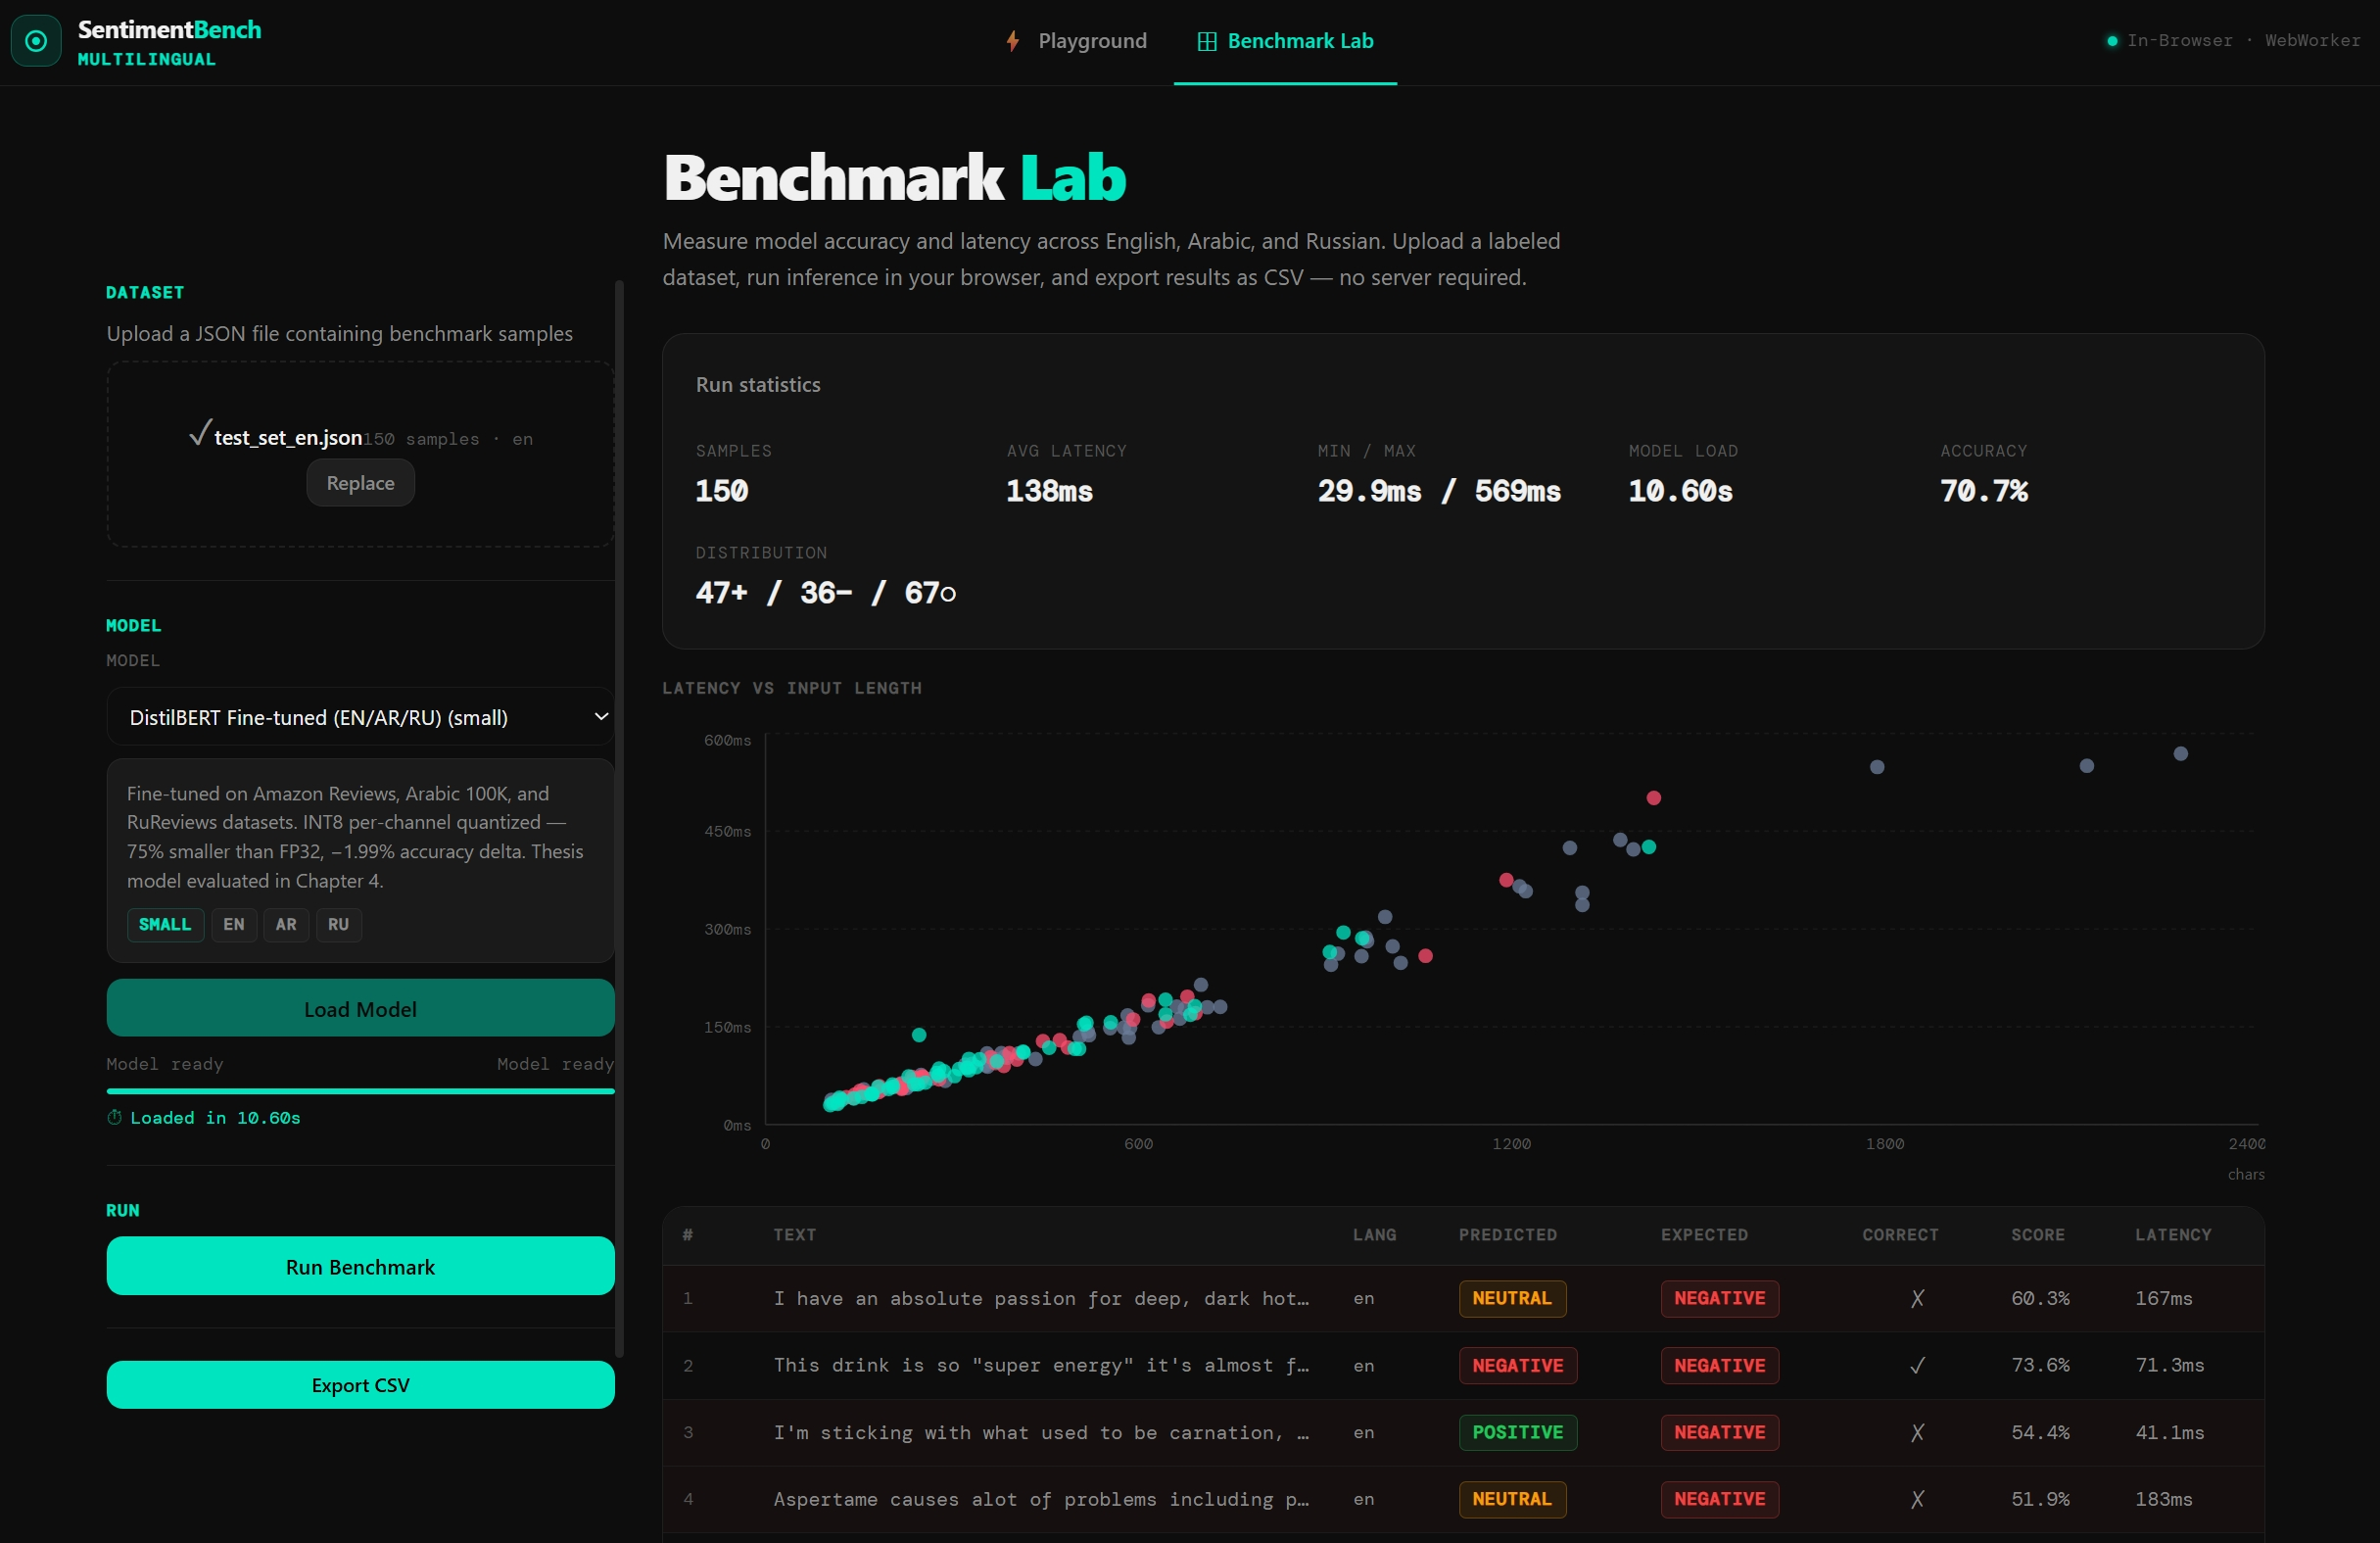
\includegraphics[width=0.95\textwidth]{images/интерфейс-лабораторного-стенда.png}
    \caption{Интерфейс режима \textit{Benchmark Lab} по завершении тестового прогона}
    \label{fig:интерфейс-лабораторного-стенда}
\end{figure}